% MDPI-format transfer adapted from paper/ACM/manuscript.tex
\documentclass[journal,article,submit,pdftex,moreauthors]{Definitions/mdpi}

\Title{Unsupervised Reference Modeling of Nanopore Signals for DNA/RNA Modification Detection}

\Author{Yongji Zou $^{1,2}$, Mian Umair Ahsan $^{1}$ and Kai Wang $^{1,3,}$*}
\AuthorNames{Yongji Zou, Mian Umair Ahsan and Kai Wang}

\address{%
$^{1}$ \quad Center for Cellular and Molecular Therapeutics, Children's Hospital of Philadelphia, Philadelphia, PA, USA; \\
$^{2}$ \quad Bioengineering Graduate Program, University of Pennsylvania, Philadelphia, PA, USA; \\
$^{3}$ \quad Department of Pathology and Laboratory Medicine, University of Pennsylvania, Philadelphia, PA, USA}

\corres{Correspondence: wangk@chop.edu}

\abstract{Nanopore sequencing produces ionic-current signals that are sensitive to chemical modifications in DNA/RNA molecules, yet accurate modification calling remains challenging due to limited labeled data and variability across experimental conditions. We present a scalable unsupervised framework for modification discovery that learns an unmodified reference signal distribution from large corpora using a CNN–Transformer variational autoencoder (VAE). The model is trained with streaming (out-of-core) random sampling and k-mer–aware soft balancing to support large-scale signal modeling. At inference, candidate nucleotides are scored using VAE reconstruction error, and read-level scores are aggregated to generate site-level evidence. On controlled DNA oligonucleotide datasets, training on unmodified sequences and testing on modified oligos yield strong discrimination. In cell line samples, training on unmodified whole-genome amplified (WGA) DNA and in vitro transcribed (IVT) RNA, and testing on natively modified (5mC/m6A) samples results in weaker performance, underscoring the difficulty of unsupervised modification calling under realistic biological noise and heterogeneity. Nevertheless, site-level anomaly score profiles display peak-like patterns that align with known modification-enriched regions. These findings demonstrate the feasibility of large-scale unsupervised reference modeling for de novo modification detection, while highlighting the challenges in translating models built from synthetic oligo datasets into robust genome-wide modification detection.}

\keyword{nanopore sequencing; base modification detection; unsupervised learning; variational autoencoder; anomaly detection}

\begin{document}

\section{Introduction}
Chemical modifications on nucleic acids, such as DNA methylation (e.g., 5-methylcytosine, 5mC) and RNA modifications (e.g., N6-methyladenosine, m6A), are central regulators of genome function and gene expression\cite{ref1}. These marks are widely implicated in development, cellular identity, and disease, and their detection at scale is an important goal in genomics. Nanopore sequencing provides a unique opportunity for modification analysis because it measures an ionic-current signal as DNA or RNA molecules pass through a nanopore; chemical modifications can induce subtle but systematic perturbations of this signal. In principle, this enables direct, single-molecule detection of diverse modifications without specialized biochemical enrichment.

In practice, accurate modification calling remains difficult. Many high-performing approaches rely on supervised learning with curated training labels. However, well-curated modification labels are scarce for many rare chemistries and can be expensive to generate at the scale needed for modern sequencing datasets. Moreover, nanopore signals are affected by sequence context, read quality, coverage variability, and experimental or computational pipelines, so models trained under one set of conditions can be brittle when applied to others. These challenges are particularly acute in scientific discovery settings, where the objective is often to prioritize candidate loci for follow-up rather than to produce a definitive genome-wide call set.

\subsection{Unsupervised reference modeling via reconstruction-based anomaly scoring}
We approach modification discovery as unsupervised reference modeling. Instead of learning a discriminative classifier from modification labels, we learn a model of unmodified nanopore signal and treat deviations as candidates for modification. Concretely, we train a CNN--Transformer variational autoencoder (VAE) on large corpora of unmodified examples, including unmodified synthetic oligos; whole-genome amplified DNA; in vitro transcribed RNA. The model aims to learn a compact latent representation that supports accurate reconstruction of canonical signal patterns across diverse sequence contexts. At inference time, we score each nucleotide instance by reconstruction error---the discrepancy between the observed signal and the model’s reconstruction---then interpreting larger errors as higher modification likelihood.

To support practical, genome-scale analyses, our training procedure is streaming/out-of-core: we sample signal windows on the fly from large read collections and optimize with stochastic mini-batches. We further incorporate soft k-mer balancing to reduce bias from skewed sequence-context frequencies and improve coverage of rare contexts. Finally, because single-read signals are noisy, we aggregate per-nucleotide anomaly scores into site-level evidence while retaining nucleotide-level resolution for advanced evaluation.

\subsection{Summary of empirical findings}
We evaluate this approach in both controlled and biological settings. Training on unmodified synthetic sequences and testing on modified oligos yields strong discrimination. In more realistic biological settings, genome-wide metrics are weaker, reflecting the difficulty of unsupervised calling under heterogeneous noise sources and variable coverage. Nevertheless, in targeted genomic regions, site-level anomaly-score profiles exhibit peak-like patterns that qualitatively track known modification profile, suggesting that the method can provide useful signal for candidate prioritization and hypothesis generation even when robust genome-wide calling remains challenging.

\subsection{Contributions}
This paper makes three contributions:
\begin{enumerate}
    \item Scalable unsupervised signal modeling. We introduce a streaming CNN--Transformer VAE framework for learning an unmodified reference distribution from large nanopore signal corpora, augmented with on-the-fly sampling and soft k-mer balancing.
    \item Reconstruction-based scoring with site aggregation. We propose a practical inference pipeline that uses reconstruction error as a per-nucleotide anomaly score and aggregates scores into site-level evidence suitable for genome-scale discovery.
    \item Evaluation across controlled and biological regimes with regional case studies. We evaluated our model on controlled modified oligos and on biological DNA/RNA datasets (WGA: native 5mC; IVT: WT m6A), and we include targeted regional analyses showing qualitative concordance between anomaly-score tracks and known modification-enriched regions.
\end{enumerate}

\section{Background and Related Work}
\subsection{Nanopore signal and modification calling}
Nanopore sequencing measures an ionic-current time series as a nucleic acid strand passes through a pore. Chemical modifications perturb this signal in a manner that depends not only on the modified base but also on local sequence context and upstream processing choices (e.g., normalization, segmentation, alignment of signal to reference). As a result, most computational methods for modified base detection can be viewed as learning (explicitly or implicitly) a mapping from signal + context to either per-read modification probabilities or per-site modification frequencies.

\subsection{Supervised and weakly supervised modified-base callers}
A large body of work performs supervised modified base calling, especially for DNA methylation, by training models on datasets with known modification states (often produced via enzymatic treatment, synthetic controls, or matched assays). Classic pipelines include HMM- or neural-network-based approaches (e.g., DeepSignal\cite{ref2}, DeepMod2\cite{ref3} and official workflows such as Guppy and Dorado\cite{ref4}), which are often benchmarked under matched conditions and can achieve strong per-read/per-site performance for common marks like 5mC at CpG sites. Systematic benchmarking efforts highlight that accuracy can depend strongly on genomic context and data characteristics, reinforcing the need for careful evaluation under realistic shifts\cite{ref5}.

For RNA modifications, supervised and weakly supervised methods typically rely on either engineered features or model architectures trained with labeled sites (or partially labeled bags of reads). For example, m6Anet\cite{ref6} uses a multiple-instance learning formulation to call m6A from direct RNA sequencing using a single sample, aiming to infer site-level modification probabilities and stoichiometry without requiring paired controls. Separately, the nanopore official caller Dorado\cite{ref4} predicts modifications anchored to canonical basecalls or reference alignments and is designed to integrate with ONT pipelines.

\subsection{“Unsupervised” and label-light approaches: paired comparisons and feature-based testing}
Alongside supervised callers, several widely used approaches are described as unsupervised or label-light because they do not require training a large discriminative model with curated labels.

One family focuses on signal-level testing against expected levels or sample-comparison statistics. Tombo\cite{ref7}, for example, provides multiple “modified base detection” strategies, including methods that test for systematic shifts in raw signal and methods that compare samples/conditions after re-squiggling (signal-to-reference alignment).

Another influential family is comparative detection, where modification evidence is derived by contrasting two matched conditions (e.g., WT vs IVT or enzyme knockout). nanoCompore\cite{ref8} is a representative framework: it detects modification-sensitive differences by comparing ionic current distributions between a sample of interest and a matched non-modified control, enabling position-level detection without a supervised training set.

These methods are powerful when (i) high-quality paired controls exist and (ii) experimental conditions are tightly coupled. However, they can be less convenient when only a single biological sample is available, when controls are expensive or imperfectly matched, or when the objective is to learn a reusable “reference” model from large, heterogeneous unmodified corpora.

\subsection{Unsupervised anomaly detection and distribution shift}
From a machine learning perspective, modification detection without dense labels is naturally connected to unsupervised representation learning and anomaly detection: learn a model of unmodified signal and score deviations as candidates. In nanopore settings, this viewpoint faces a distinctive challenge: the observed signal distribution can shift substantially across regimes (synthetic oligos vs whole-genome DNA vs cellular RNA; WGA vs native; even different runs/chemistries/basecallers), so “anomalous” may reflect domain shift as much as true chemical modification. Empirically, this motivates both (1) modeling choices that can scale to large unmodified datasets and (2) evaluation protocols that explicitly probe transfer across experimental regimes rather than assuming in-distribution generalization.

\section{Problem Setup}
\subsection{Inputs and notation}
We consider nanopore reads aligned to a reference genome (DNA) or transcriptome (RNA). Let $j$
index a \emph{reference site}, i.e., a genomic/transcriptomic coordinate (chromosome/transcript,
position, and strand). Let $\mathcal{R}_j$ denote the set of reads covering site $j$.

For each read $r \in \mathcal{R}_j$, we construct a fixed-length, per-nucleotide \emph{instance}
centered at the nucleotide aligned to site $j$, represented by a feature tensor
\begin{equation}
x_{r,j} \in \mathbb{R}^{L \times C},
\end{equation}
where $L$ is the window length (timesteps/positions in the window) and $C$ is the number of
feature channels (signal-derived + auxiliary features). The window implicitly encodes local context,
and we additionally associate each instance with an explicit $k$-mer context (derived from the
reference) used for sampling/balancing during training.

Our goal is to output:
\begin{enumerate}
    \item an \textbf{instance-level} (per-read, per-site) anomaly score $s_{r,j}$ indicating how much
    $(r,j)$ deviates from an \emph{unmodified reference model}, and
    \item a \textbf{site-level} score $S_j$ summarizing modification evidence at reference site $j$
    by aggregating instance-level scores over reads.
\end{enumerate}

\subsection{Unsupervised reference modeling with a VAE}
We assume access to an \emph{unmodified} training corpus $\mathcal{D}_0$ (e.g., unmodified oligos,
WGA DNA, or IVT RNA), intended to represent canonical (unmodified) signal under a given regime.
We train a variational autoencoder (VAE) with decoder $p_\theta(x \mid z)$ and encoder
$q_\phi(z \mid x)$ to model the distribution of unmodified inputs:
\begin{equation}
\min_{\theta,\phi}\; \mathbb{E}_{x \sim \mathcal{D}_0}\left[\mathcal{L}_{\mathrm{VAE}}(x; \theta,\phi)\right].
\end{equation}
We use the standard negative-ELBO objective:
\begin{equation}
\mathcal{L}_{\mathrm{VAE}}(x)
=
\underbrace{\ell\!\left(x,\hat{x}\right)}_{\text{reconstruction}}
+
\beta\;
\underbrace{\mathrm{KL}\!\left(q_\phi(z \mid x)\;\|\;p(z)\right)}_{\text{regularization}},
\end{equation}
where $p(z)=\mathcal{N}(0,I)$, $\hat{x}$ is the reconstruction, $\ell(\cdot,\cdot)$ is mean-squared
error (MSE), and $\beta$ controls the KL term.

\subsection{Instance-level anomaly scoring}
Given a trained model, we compute an anomaly score for each nucleotide instance $(r,j)$ using
reconstruction error:
\begin{equation}
s_{r,j} = \ell\!\left(x_{r,j}, \hat{x}_{r,j}\right).
\end{equation}
Intuitively, if $x_{r,j}$ deviates from the learned unmodified manifold (e.g., due to a chemical
modification or other systematic perturbation), reconstruction error tends to increase. This yields a
continuous score suitable for candidate ranking.

\subsection{Site-level aggregation and reliability summaries}
To obtain site-level evidence, we aggregate instance scores across reads covering site $j$:
\begin{equation}
S_j = \mathrm{Agg}\left(\left\{ s_{r,j} : r \in \mathcal{R}_j \right\}\right).
\end{equation}
We consider simple robust aggregators such as mean and median. In addition to $S_j$, we compute
coverage and dispersion summaries (e.g., $n_j = |\mathcal{R}_j|$, standard deviation/MAD of
$\{s_{r,j}\}$, and standard error of the mean) to contextualize confidence as a function of coverage
and noise, and to enable coverage-aware reporting or thresholding when desired.

\subsection{Labels for evaluation}
Training is fully label-free. For evaluation, we use reference labels when available:
instance-level $y_{r,j}\in\{0,1\}$ and site-level $Y_j\in\{0,1\}$ for designed oligos, and
high-quality reference tracks (e.g., Dorado calls) as pseudo-labels in biological datasets.
We evaluate both instance- and site-level discrimination because they support different use cases:
read-level analyses/stoichiometry vs.\ robust site-level discovery.

\section{Methods}
\subsection{Overview}
We learn an unmodified reference distribution of nanopore signal instances using a CNN--Transformer
VAE trained on unmodified corpora. Training is performed in a streaming (out-of-core) manner by
sampling windows on the fly from large aligned read files. At inference time, we use reconstruction
error as an instance-level anomaly score and aggregate across reads to produce site-level evidence.

\subsection{Input representation and feature construction}
For each aligned nucleotide instance $(r,j)$ we extract a fixed-length window centered on the
aligned position and construct a feature tensor $x_{r,j}\in \mathbb{R}^{L\times C}$.

\paragraph{Signal windowing and normalization.}
We use a local window around the aligned nucleotide to capture the focal base and neighboring
context. Raw current is normalized per read using standard $z$-normalization to reduce
run-to-run amplitude variation.

\paragraph{Auxiliary feature channels.}
In addition to one-hot base identity, we include event-/window-level summary features (Table~1 in
the manuscript), yielding $C=11$ channels in our primary configuration (base identity, winsorized
mean, quartiles, central signal value, RMS energy, and basecaller quality).

\paragraph{Sequence context (k-mers).}
Each instance is associated with a reference-derived $k$-mer (default $k=7$) used for soft balancing
during streaming. The $k$-mer is not required for VAE reconstruction but helps reduce sampling bias
from highly imbalanced context frequencies.

\subsection{CNN--Transformer VAE architecture}
We model $x_{r,j}$ using a CNN--Transformer VAE. The CNN encoder captures local signal morphology,
while the Transformer captures dependencies across timesteps within the window.

\paragraph{Encoder.}
The encoder applies 1D convolutional blocks to map $x_{r,j}$ into a token sequence, adds positional
encoding, and passes tokens through a Transformer encoder. A pooling operation produces a
fixed-length representation $h_{r,j}$, which parameterizes a diagonal Gaussian posterior:
\begin{equation}
q_\phi(z\mid x) = \mathcal{N}\!\left(\mu_\phi(x),\mathrm{diag}(\sigma_\phi^2(x))\right).
\end{equation}

\paragraph{Decoder.}
The decoder maps $z$ back to a reconstructed window $\hat{x}_{r,j}\in\mathbb{R}^{L\times C}$ via a
latent-to-token projection followed by Transformer blocks and a lightweight convolutional head.

\paragraph{Objective.}
We optimize the negative ELBO (Eq.\ in Problem Setup) with reconstruction MSE and a $\beta$-weighted
KL term, using $\beta$ warm-up during early epochs to improve stability.

\subsection{Streaming training with on-the-fly sampling}
Nanopore signal corpora are too large to materialize as conventional in-memory datasets. We train
out-of-core by sampling training instances directly from aligned read files.

\paragraph{On-the-fly random sampling.}
Each optimization step draws a mini-batch by randomly selecting reads and aligned positions, then
extracting windows and constructing $x_{r,j}$ online. This produces a stochastic training stream and
improves coverage over large corpora.

\paragraph{Soft $k$-mer balancing.}
To mitigate extreme imbalance in sequence-context frequencies, we apply a soft acceptance scheme
that down-weights over-represented $k$-mers during streaming. Let $N_{\text{seen}}(u)$ denote the
number of accepted instances so far for $k$-mer $u$ (tracked online). We accept a candidate instance
with probability
\begin{equation}
p_{\text{accept}}(u) = \min\!\left(1,\; \frac{C_{\max}}{N_{\text{seen}}(u)+1}\right),
\end{equation}
where $C_{\max}$ is a global soft cap controlling how quickly acceptance decays for frequent contexts.
This scheme preserves diversity without imposing hard stratification.

\paragraph{Optimization details.}
We train using AdamW with standard regularization, $\beta$ warm-up in early epochs, and early
stopping on an unmodified validation subset. The final hyperparameters and model checkpoints are
reported in the accompanying code release.

\begin{figure}[t]
\centering
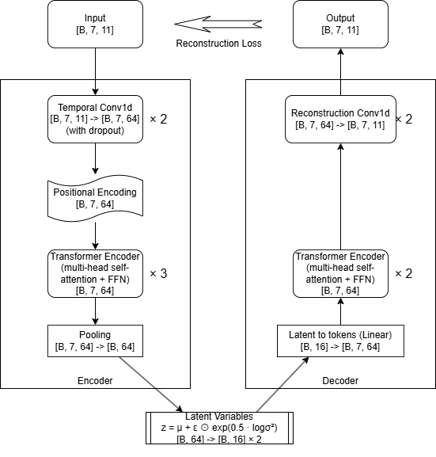
\includegraphics[width=\linewidth]{figures/figure1.png}
\caption{CNN--Transformer VAE architecture for nanopore signal window modeling. Each training instance is a length-7 window with 11 input features, represented as a tensor [B,7,11]. The encoder applies a temporal 1D convolution (with dropout) to map features to a 64-dimensional token space [B,7,64], adds positional encodings, and passes tokens through a Transformer encoder. A pooling operation produces a fixed-length latent representation (parameterized as a VAE latent of dimension 16). The decoder projects the latent back to token space (“latent-to-tokens”), applies a Transformer encoder block, and uses a reconstruction Conv1D head to recover the original feature tensor [B,7,11]. Reconstruction error is used as the per-nucleotide anomaly score and can be aggregated across reads for site-level evidence.}
\label{fig:1}
\end{figure}

\section{Experimental Design}
\subsection{Datasets and evaluation settings}
We evaluate in two complementary settings: (i) controlled synthetic oligonucleotides with designed modification positions and (ii) biological datasets using unmodified proxies for training and native samples for evaluation.

Controlled oligonucleotides (DNA/RNA). Oxford Nanopore released some of their synthetic oligos data\cite{ontOligos}. We use unmodified oligos as training data and evaluate on modified oligos containing known modification types (e.g., 5mC for DNA and m6A for RNA). Because modified positions are designed, both per-nucleotide and per-site labels are available, enabling clean benchmarking of sensitivity.

Biological DNA: HG002 WGA v.s HG002 native methylation. We train on HG002 whole-genome amplified (WGA) DNA (used as an unmodified proxy) and evaluate on native HG002 DNA containing endogenous methylation (5mC). We report per-site evidence after aggregation to compare with the modification labels generated by SOTA supervised model (Dorado).

Biological RNA: IVT v.s WT m6A modification. We generated and sequenced our own wild-type (WT) and in vitro transcribed (IVT) data for HEK293T cell line. We train on IVT RNA (unmodified proxy) and evaluate on WT direct RNA samples containing m6A. We report per-site evidence after aggregation to compare with the modification labels generated by SOTA supervised model (Dorado).

\subsection{Preprocessing and instance construction}
All datasets are processed through a common pipeline to obtain aligned read coordinates and per-instance signal windows.

Basecalling and alignment. Reads are basecalled using the best models from Dorado and aligned to the reference human or synthetic genome/transcriptome using Minimap2. Signal windows are assigned to reference positions using event segmentation and alignment (“re-squiggling”) based on the “move table” output from Dorado.

Signal embedding to BAM. Raw sequencing pod5 files are analyzed and embedded in the aligned BAM files to create an unified data input format to use in model training. Original electric squiggles as well as general basecalling and alignment information can be accessed uniformly from the embedded “SignalBAM” file.

Window extraction. For each nucleotide instance from each read, we extract a fixed-length signal window centered on the aligned position and apply normalization and feature construction as described in Methods.

\subsection{Metrics}
We report both instance-level and site-level metrics.

Instance-level (per-nucleotide). AUROC for discrimination between modified and unmodified instances (where instance labels exist).

Site-level (per-site). AUROC for site classification after aggregation. Average precision (AP/AUPRC) when prevalence is not extreme, and labels are reliable.

\subsection{Regional case studies: concordance with known modification-enriched regions}
To assess whether anomaly scores capture biologically meaningful structure beyond global metrics, we select several genomic regions with known modification enrichment (peak regions from curated Dorado tracks). For each region, we visualize the site-level anomaly score  as a genome track and compare its peak-like structure to the known modification-enriched signal.

We also report qualitative concordance (visual alignment of peaks) and optionally summarize each region with a simple quantitative statistic such as (i) Spearman correlation between smoothed anomaly-score and peak tracks across bins or (ii) overlap/enrichment of top-scoring sites within annotated peaks. Within each region, positives are positions inside Dorado peak intervals; negatives are positions outside peaks but within the same region after excluding low-coverage sites.

\subsection{Implementation details}
We train all models using one A100 GPU with 20 CPUs, and roughly 20 epochs on the unmodified training corpus, selecting hyperparameters on a held-out unmodified validation subset.

\section{Results}
We evaluate reconstruction-error--based unsupervised reference modeling in (i) controlled synthetic oligonucleotides with designed modifications and (ii) biological datasets where unmodified proxies (WGA DNA; IVT RNA) are used for training and native samples are used for evaluation. Unless otherwise stated, per-site scores are computed by mean aggregation across reads, and per-nucleotide scores correspond to instance-level reconstruction error as defined in Section 3.

\subsection{Controlled DNA oligos: strong per-nucleotide discrimination and near-perfect site aggregation}

Setup. We train on unmodified synthetic DNA oligos and test on modified oligos with known modified positions. This setting provides clean per-nucleotide and per-site ground truth, enabling direct assessment of modification sensitivity independent of biological confounders.

5mC (CpG) oligos. The model achieves strong per-nucleotide discrimination for 5mC at the instance level (AUROC = 0.859; AUPRC = 0.837). Aggregating instance scores to the reference site level yields near-perfect performance (AUROC = 0.991; AUPRC/AP = 0.991), indicating that site-level evidence becomes highly reliable once per-read noise is averaged out (Figure 2).

5hmC (CpG) oligos. We further evaluate on additional modified oligos (5hmC) (Supp Figure 1). While these chemistries may induce different magnitudes and shapes of perturbations, the same reconstruction-error scoring pipeline applies unchanged. The model also achieves strong per-nucleotide discrimination at the instance level (AUROC = 0.854; AUPRC = 0.826). Similarly, aggregating instance scores to the reference site level yields near-perfect performance (AUROC = 0.991; AUPRC/AP = 0.991).

\begin{figure}[t]
\centering
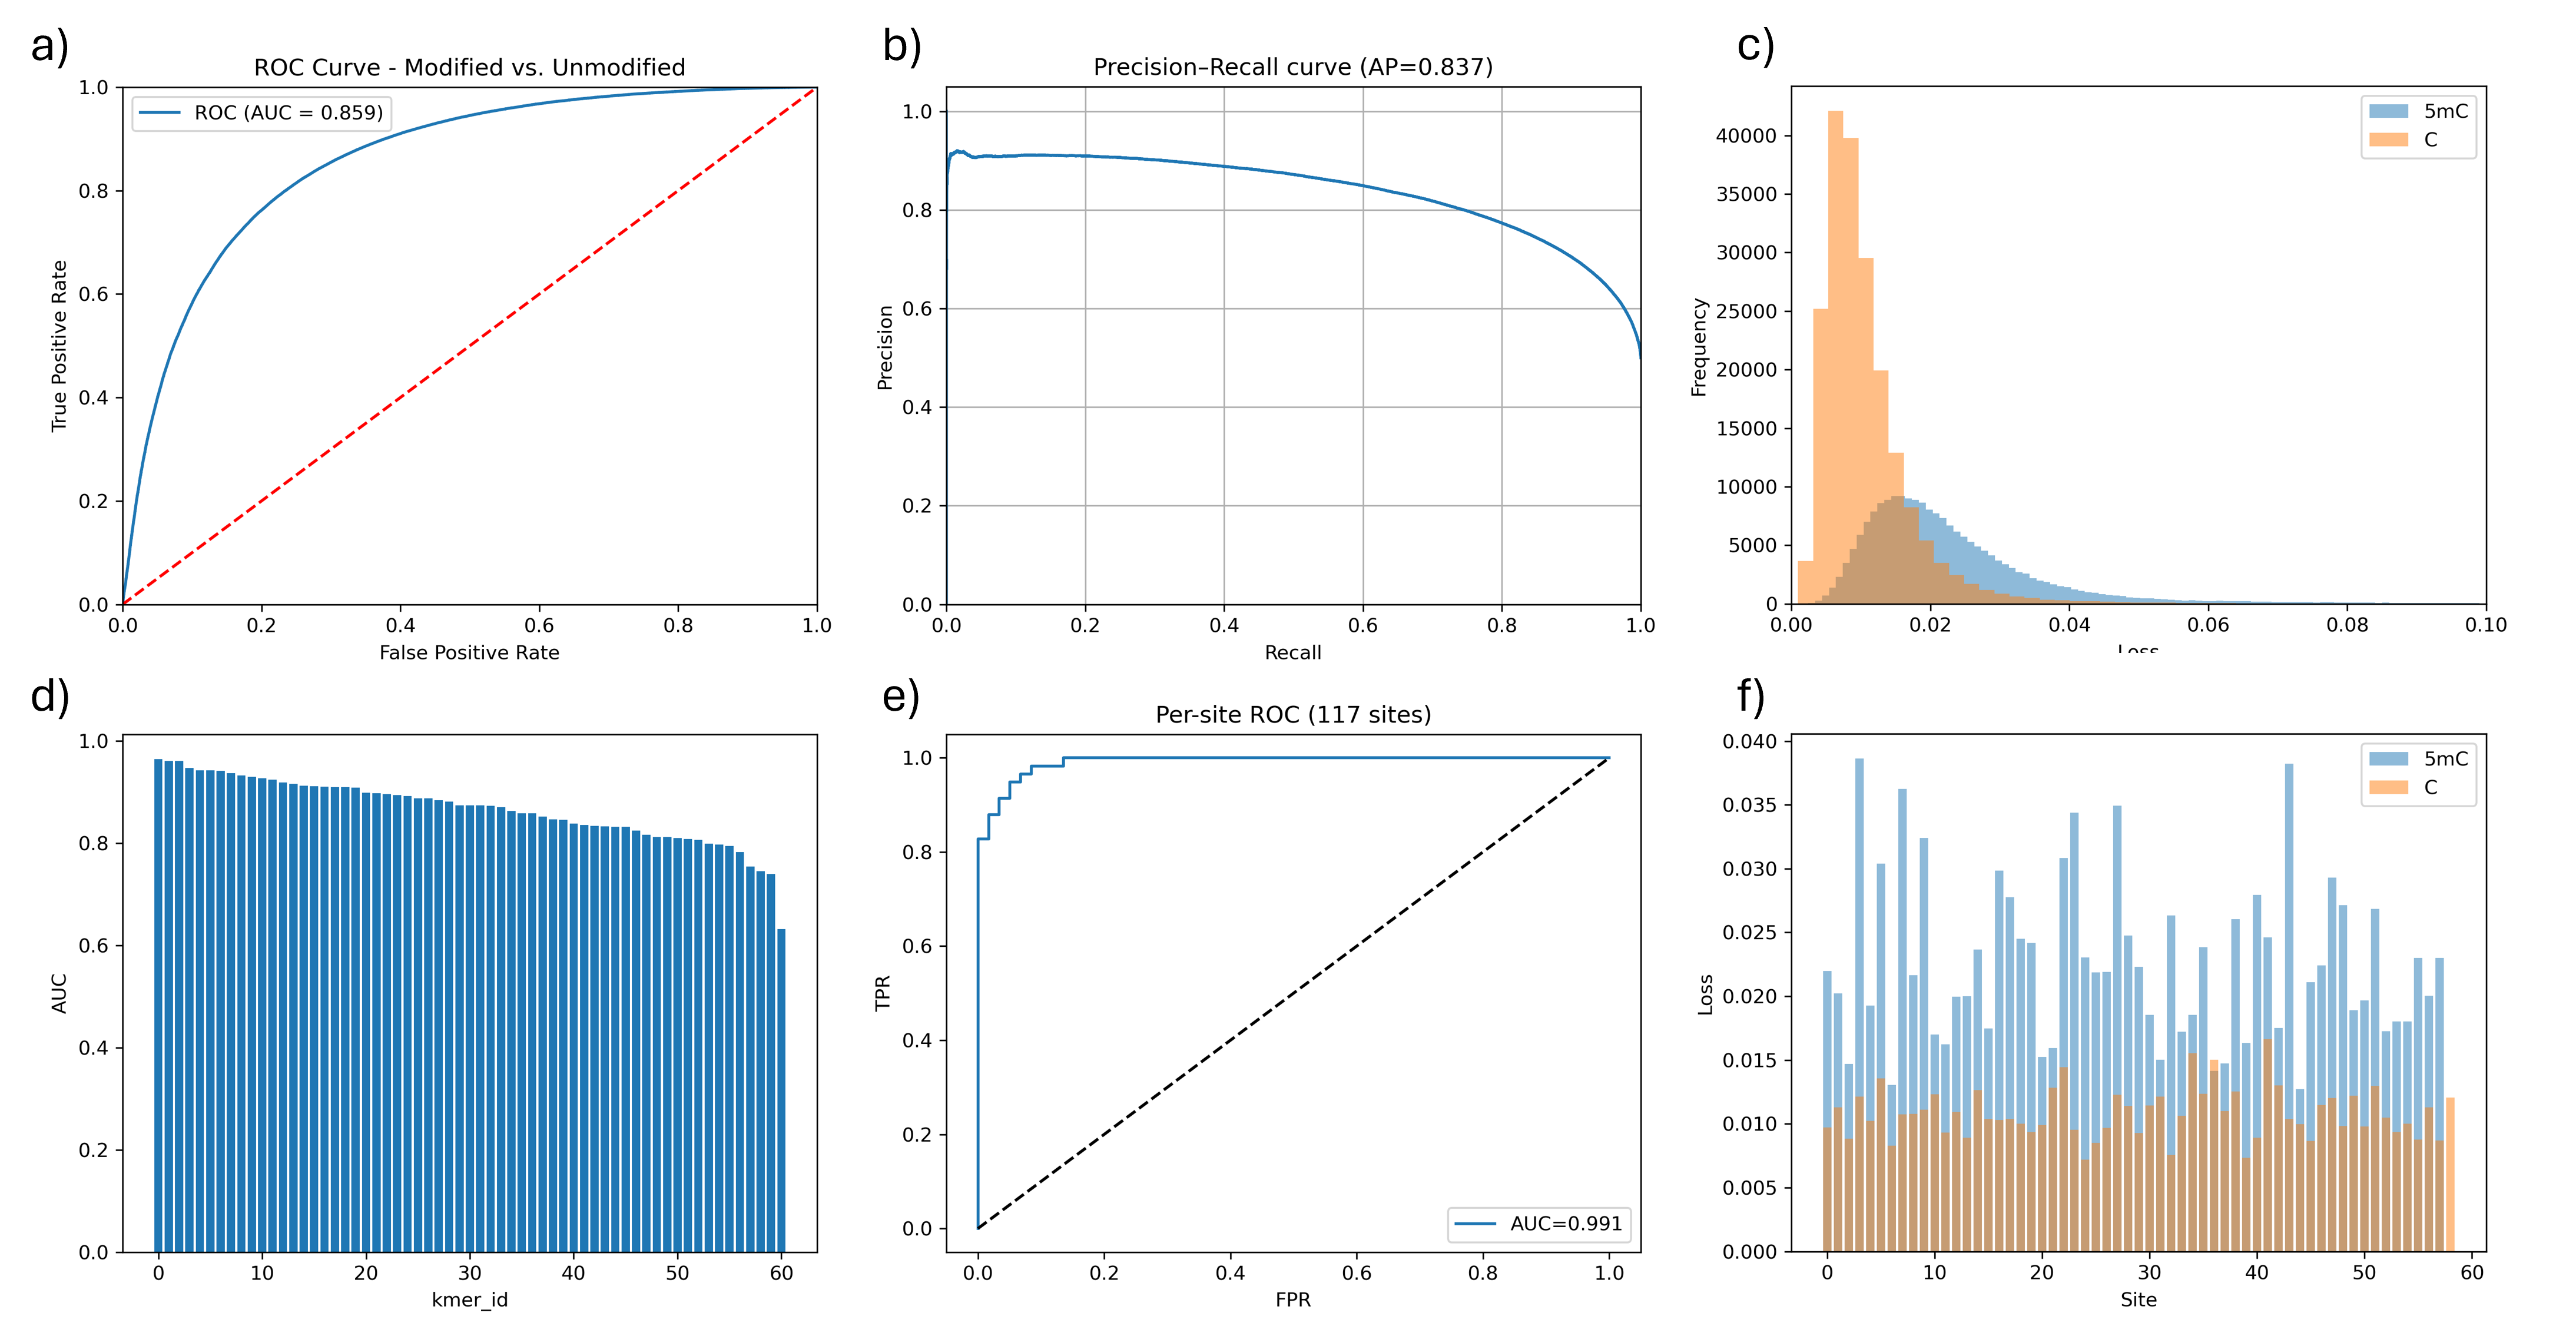
\includegraphics[width=\linewidth]{figures/figure2.png}
\caption{Controlled 5mC oligo evaluation of reconstruction-error anomaly scoring at nucleotide and site levels. (a) Per-nucleotide ROC curve for modified vs. unmodified instances (AUROC = 0.859; dashed line indicates random baseline). (b) Per-nucleotide precision--recall curve (AUPRC/AP = 0.837). (c) Distribution of per-nucleotide reconstruction loss for modified (5mC) and unmodified (C) bases, showing a right-shift for modified instances. (d) Per-k-mer AUROC across sequence contexts, indicating performance variability by local k-mer. (e) Per-site ROC computed after aggregating per-nucleotide scores across reads for each site (117 sites; AUROC = 0.991). (f) Site-level mean reconstruction loss for modified vs. unmodified sites, illustrating consistent separation after aggregation.}
\label{fig:2}
\end{figure}

\subsection{Biological DNA: HG002 WGA → native HG002 5mC}
Setup. We train on HG002 whole-genome amplified (WGA) DNA as an unmodified proxy and evaluate on native HG002 DNA containing endogenous 5mC. Site-level labels for evaluation are derived from Dorado modification calls, which we use as a reference track rather than definitive ground truth.

Genome-wide performance. In this more realistic regime, discrimination decreases relative to controlled oligos, showing a drop from the oligo setting. We report:

per-nucleotide: AUROC = 0.638; AUPRC = 0.610

per-site: AUROC = 0.639; AUPRC/AP = 0.629 (Figure 3).

Interpretation. The reduction from the controlled setting is consistent with additional sources of variability in whole-genome data (coverage heterogeneity, broader sequence-context diversity, and run/pipeline artifacts). Notably, the model still provides a meaningful ranking of candidate sites, supporting its use in prioritization workflows.

\begin{figure}[t]
\centering
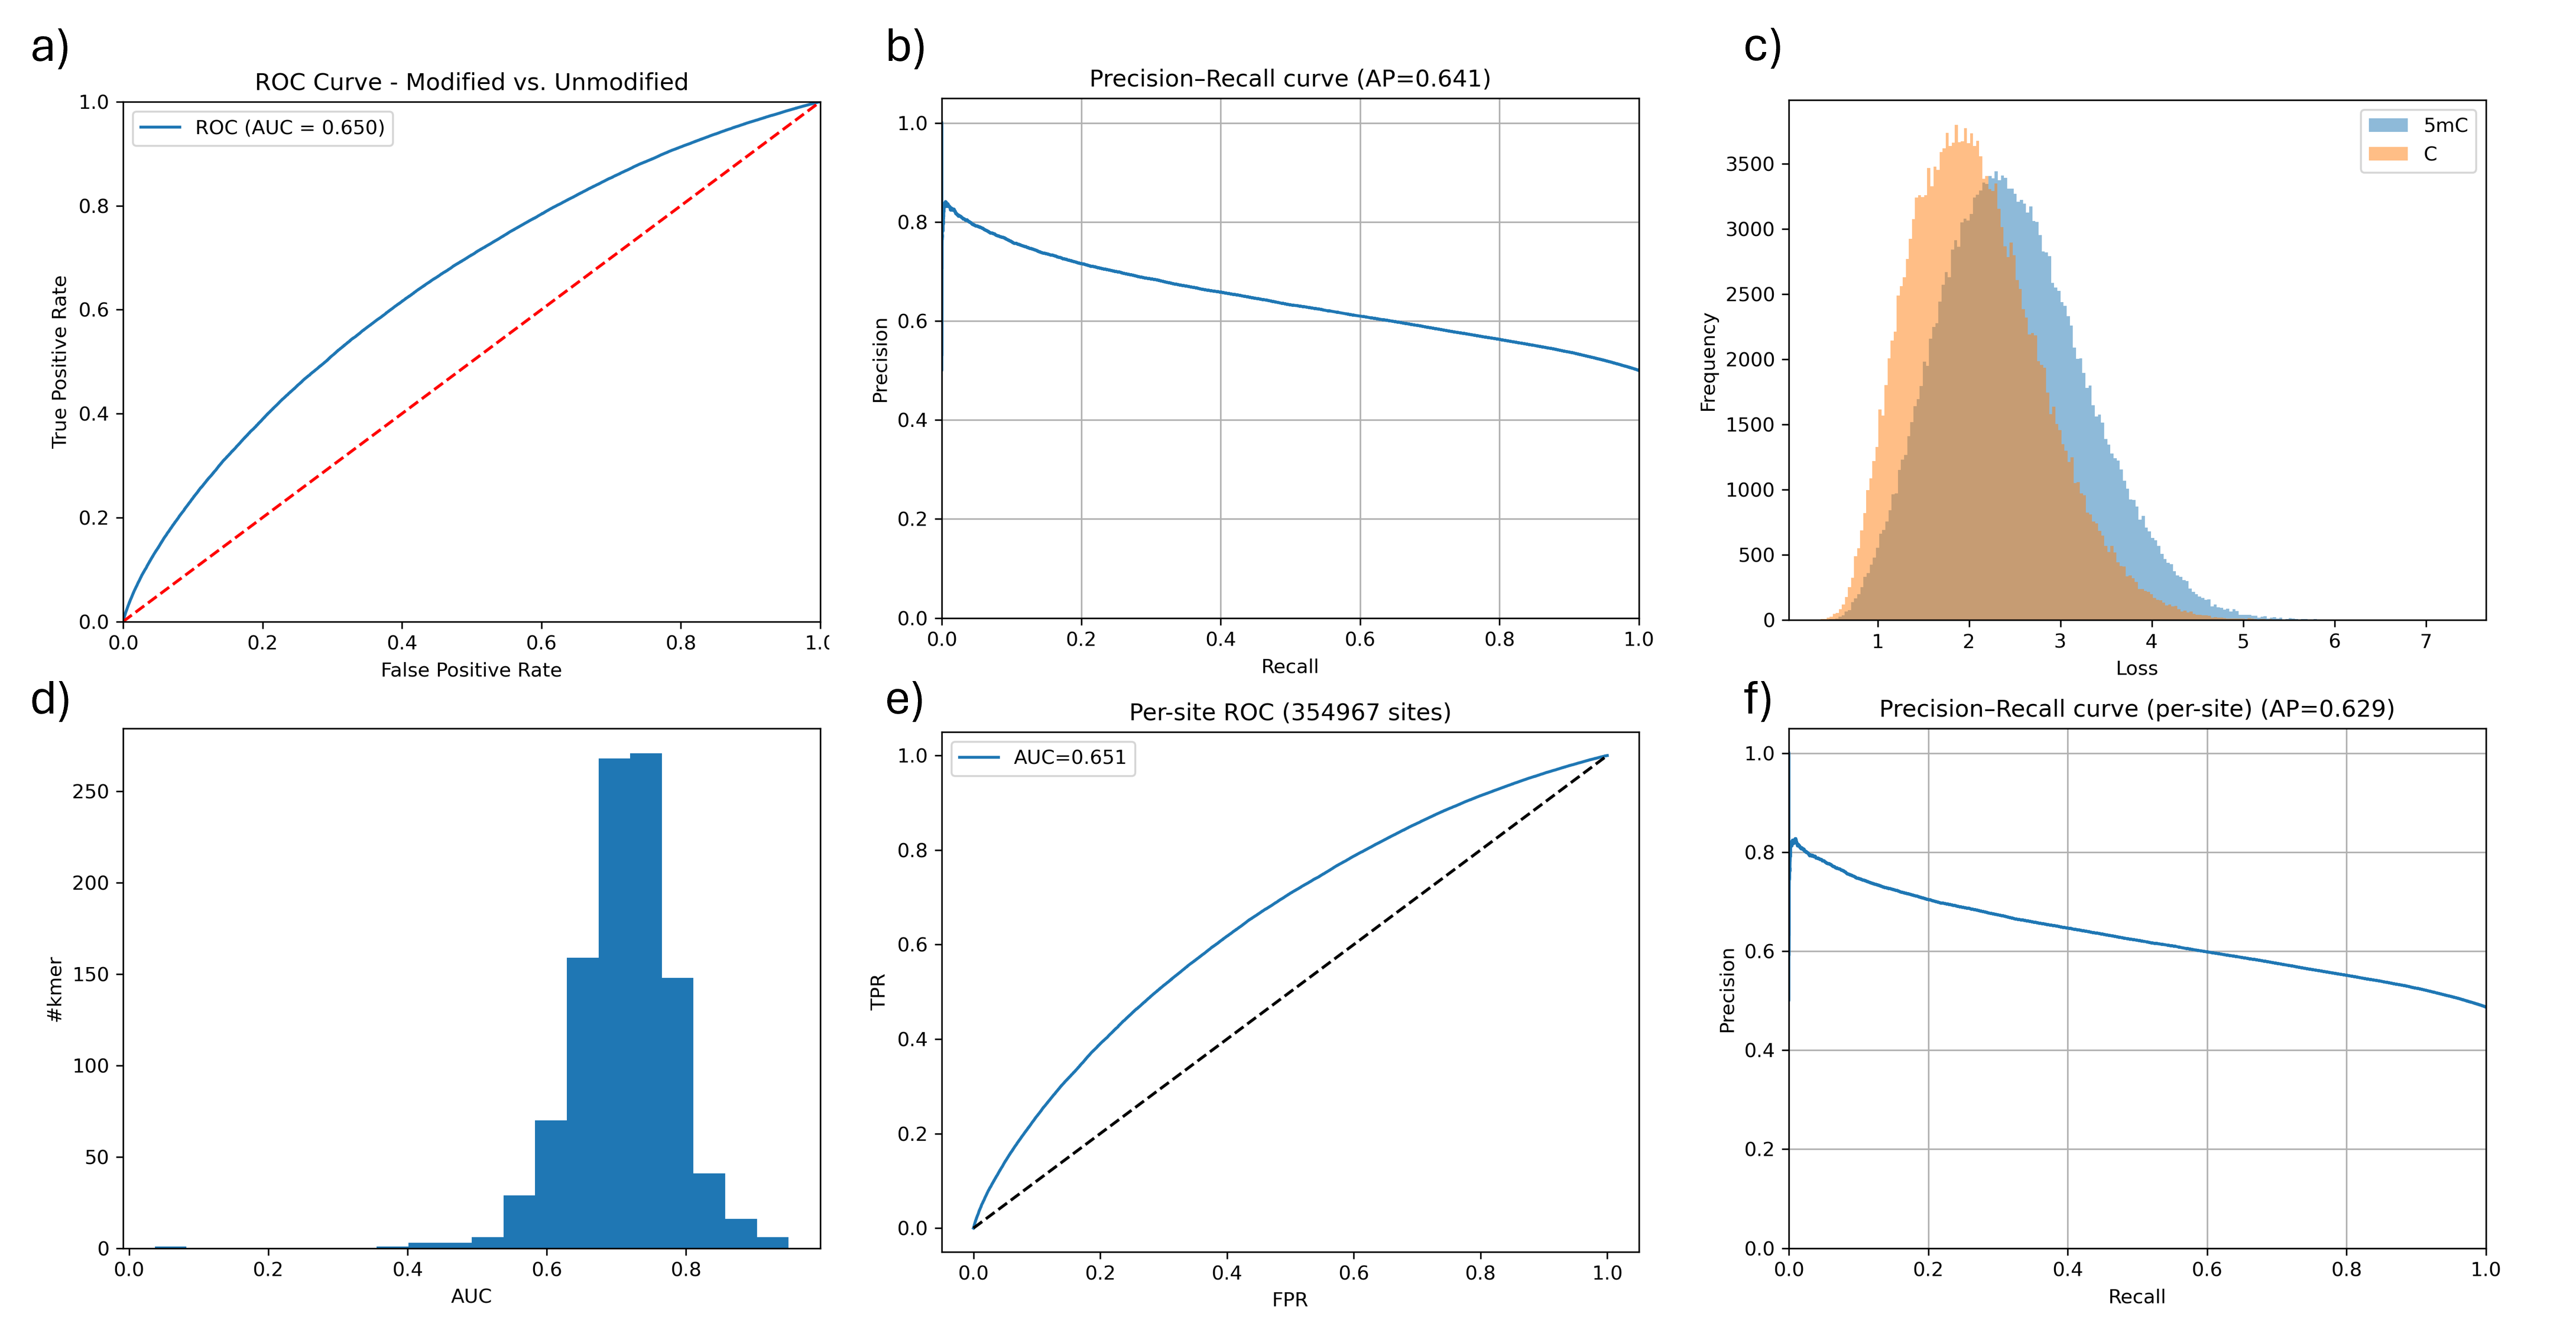
\includegraphics[width=\linewidth]{figures/figure3.png}
\caption{Whole-genome evaluation on HG002: WGA (unmodified proxy) → native 5mC using reconstruction-error anomaly scoring. (a) Per-nucleotide ROC curve for modified vs. unmodified instances (AUROC = 0.650; dashed line indicates random baseline). (b) Per-nucleotide precision--recall curve (AUPRC/AP = 0.641). (c) Distribution of per-nucleotide reconstruction loss for 5mC and unmodified C bases, showing partial separation and substantial overlap under biological heterogeneity. (d) Histogram of per-k-mer AUROC values across sequence contexts, illustrating context-dependent variability in genome-wide performance. (e) Per-site ROC after aggregating per-nucleotide scores across reads for each genomic site (354,967 sites; AUROC = 0.651). (f) Per-site precision--recall curve (AUPRC/AP = 0.629), reflecting ranking utility despite modest discrimination at scale.}
\label{fig:3}
\end{figure}

\subsection{Biological RNA: IVT → WT m6A in HEK293T}
Setup. We generate direct RNA sequencing data for HEK293T wild-type (WT) RNA and a matched in vitro transcribed (IVT) RNA dataset. We train on IVT as an unmodified proxy and evaluate on WT, using Dorado m6A calls as the reference track for evaluation.

Genome-wide performance under heavy class imbalance. We observe AUROC = 0.592 at the per-nucleotide level (Supp Figure 2). Because m6A positives are extremely sparse genome-wide, AUPRC/AP is over dominated by prevalence and label noise.

Interpretation. These results indicate weak signal at the instance level, highlight the difficulty of achieving strong genome-wide calling performance without additional calibration and shift-handling in complex RNA samples.

\subsection{Regional case studies: anomaly-score tracks align with modification-enriched peaks}
Global metrics can understate utility in discovery workflows, where the goal is often to prioritize candidate regions and sites. We therefore examine whether site-level anomaly scores produce biologically meaningful spatial patterns along the genome or transcriptome.

Method. For selected regions with strong modification enrichment in the Dorado reference tracks, we visualize the site-level anomaly score profile (mean aggregated across reads) and compare it to the modification peak structure.

Findings. Across multiple regions, anomaly-score profiles exhibit peak-like structure that qualitatively follows known modification-enriched regions (Figure 4). This concordance suggests that reconstruction-based reference modeling can capture spatially coherent modification signals even when genome-wide discrimination remains modest.

Quantitative summaries. Where applicable, we summarize concordance using region-level statistics such as Spearman correlation between binned/smoothed anomaly scores and reference peak tracks (e.g., $\rho = 0.342$ for one representative region; Figure 4). We also define the exact positive/negative labeling for these region-level ROC/PR analyses (e.g., Dorado peak vs non-peak positions) in order to quantify the concordance.

\begin{figure}[t]
\centering
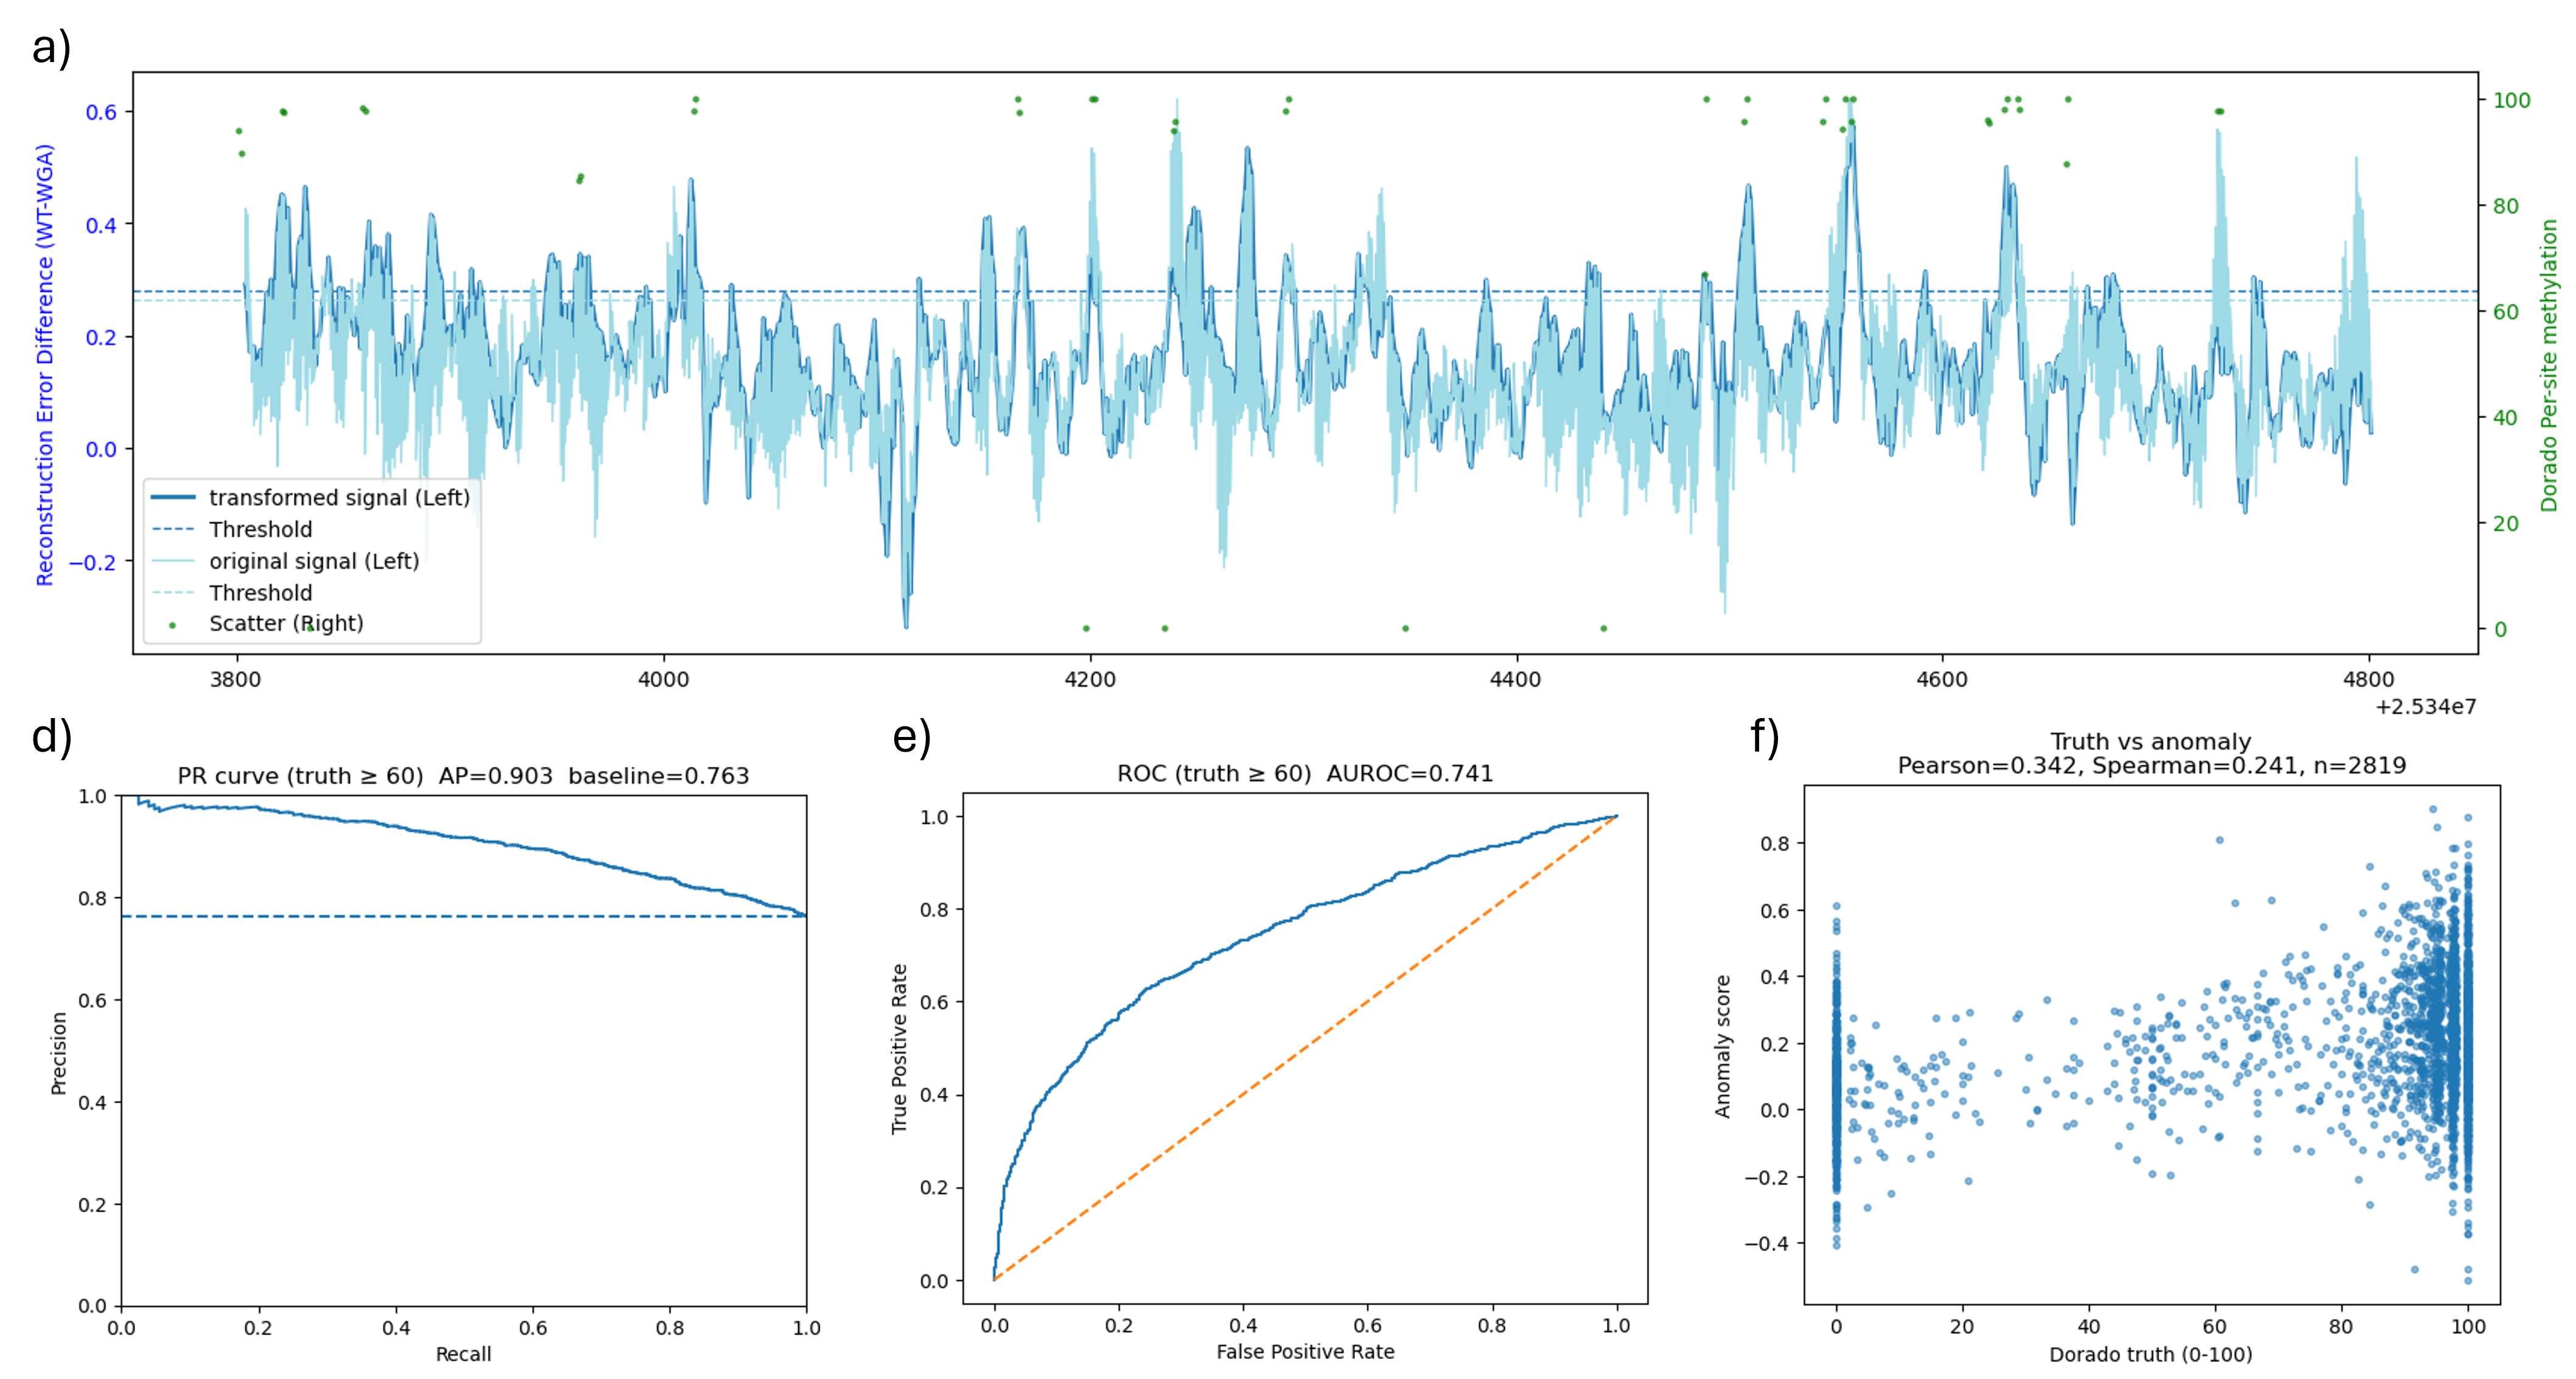
\includegraphics[width=\linewidth]{figures/figure4.png}
\caption{Regional case study: site-level anomaly scores track methylation-enriched peaks in native HG002. (a) Anomaly score profile (difference in mean reconstruction error between WT and WGA) plotted along a representative genomic region (left y-axis), overlaid with Dorado per-site methylation levels (green markers; right y-axis). Horizontal dashed lines indicate thresholds used for visualization/region-level evaluation. (b) Precision--recall curve for classifying positions within the region using anomaly scores, with positives defined as sites exceeding a Dorado methylation threshold (truth $\geq 60$; AP $= 0.903$; dashed line shows prevalence baseline $= 0.763$). (c) ROC curve for the same regional classification task (truth $\geq 60$; AUROC $= 0.741$; dashed line indicates random baseline). (d) Scatter plot comparing Dorado methylation levels (0-100) to anomaly scores across sites in the region (n $= 2819$), showing moderate correlation (Pearson $= 0.342$; Spearman $= 0.241$).}
\label{fig:4}
\end{figure}

\subsection{Summary}
Controlled oligo experiments demonstrate strong sensitivity of reconstruction-error scoring to modification-induced signal perturbations, with near-perfect performance after site-level aggregation. In biological DNA/RNA settings, genome-wide metrics are weaker under realistic noise and heterogeneity, but regional analyses show peak-like alignment between anomaly-score tracks and modification-enriched regions. Together, these results support unsupervised reference modeling as a practical, label-light approach for candidate prioritization and hypothesis generation while motivating future work on calibration and robustness for genome-wide calling.

\section{Discussion}
Our results indicate that reconstruction-based unsupervised reference modeling provides a practical and adaptable framework for nanopore modification discovery. The approach performs strongly under controlled conditions and shows emerging utility in biological datasets when used for prioritization and exploratory analysis rather than definitive site calling.

\subsection{Current Utility and Use Cases}
\paragraph{Prioritization under limited supervision.}
A key advantage of reference modeling is that it does not require dense modification labels for training. In regimes where labels are unavailable, incomplete, or costly to obtain, reconstruction-error scores provide a continuous ranking signal that can guide downstream validation and targeted follow-up.

\paragraph{Hypothesis generation and regional discovery.}
Even when genome-wide discrimination is modest in biological samples, regional analyses suggest that aggregated anomaly-score profiles can exhibit spatially coherent patterns that align qualitatively with modification-enriched intervals. This supports discovery-oriented use cases in which contiguous signal, rather than per-site certainty, is informative—for example, nominating candidate loci, transcripts, or genomic intervals for follow-up experiments.

\subsection{Methodological Improvements and Validation Priorities}
\paragraph{Handling domain shift and calibration.}
The performance gap between controlled oligos and biological datasets suggests that covariate shift and heterogeneous noise sources can obscure modification-associated signal. Promising directions include shift-aware normalization (e.g., run/kit/basecaller effects), coverage-aware calibration of score distributions, and aggregation schemes that better accommodate partial occupancy and outlier reads.

\paragraph{Reproducibility across runs and laboratories.}
For deployment, it is critical that anomaly scores remain stable across sequencing runs, flow cells, and pipeline versions. Multi-run and multi-laboratory evaluations—paired with transparent reporting of preprocessing and parameter choices—would help quantify reproducibility and establish best practices.

\paragraph{Preprocessing control and documentation.}
Reconstruction-based scoring is sensitive to the input representation. Changes in basecalling, signal-to-reference mapping, normalization, or feature extraction can shift the learned reference distribution and thus the resulting score scale. We therefore recommend using consistent preprocessing within a study and reporting tool versions and key parameters to support reproducibility.

\paragraph{Characterizing failure modes.}
Elevated anomaly scores can reflect non-biological artifacts (e.g., alignment ambiguity, low-quality reads, signal drift) in addition to chemical modifications. Incorporating QC filters and stratified analyses by read quality, mapping quality, and coverage can reduce spurious discoveries and clarify the conditions under which the method is reliable.

\section{Limitations and Ethical Considerations}
\paragraph{Genome-wide performance in biological samples.}
Although controlled oligos exhibit strong sensitivity and site-level aggregation yields near-ceiling performance, genome-wide discrimination in biological DNA/RNA remains comparatively modest. Consequently, the current method is better suited to prioritization and exploratory analyses than to comprehensive genome-wide annotation as a standalone caller.

\paragraph{Dependence on preprocessing choices and proxy references.}
The approach assumes access to an unmodified proxy dataset (e.g., WGA DNA or IVT RNA) and depends on signal-to-reference mapping and normalization decisions. Differences in preprocessing pipelines can alter the learned reference distribution and, in turn, change anomaly-score distributions and thresholds.

\paragraph{Limited robustness characterization across domains.}
Our experiments do not yet exhaustively assess variability across flow cells, library preparations, basecaller versions, or laboratories. Therefore, claims regarding cross-domain robustness should be interpreted cautiously until broader evaluations are performed.

\paragraph{Potential bias across datasets and populations.}
Performance may vary with sample composition, ancestry-linked genomic variation, and experimental protocols. Reporting dataset composition and evaluating across diverse samples can help identify and mitigate such biases, improving generalizability and responsible use.

\section{Conclusion}
We presented a scalable, label-light framework for nanopore modification discovery based on unsupervised reference modeling with a streaming CNN--Transformer VAE. By scoring reconstruction error as an anomaly signal and aggregating per-nucleotide evidence into site-level summaries, the method achieves strong discrimination in controlled DNA/RNA oligo benchmarks and reveals biologically meaningful, peak-like anomaly patterns in selected genomic regions of wild-type samples. Although genome-wide performance in complex biological datasets remains challenging, these results support reconstruction-based reference modeling as a practical approach for candidate prioritization and hypothesis generation, and motivate future work on shift-handling, calibration, and robust biological validation to enable reliable genome-wide calling.

\section*{Generative AI Disclosure}
Generative AI tools (ChatGPT) were used to assist with language polishing and \LaTeX{} formatting of this manuscript. All scientific content, experimental design, analysis, and conclusions were developed by the authors, who reviewed and approved the final text.

\begin{adjustwidth}{-\extralength}{0cm}
\reftitle{References}
\begin{thebibliography}{99}
\bibitem{ref1}
Delaunay S, Helm M, Frye M: RNA modifications in physiology and disease: towards clinical applications. Nature Reviews Genetics 2024, 25(2):104-122.

\bibitem{ref2}
Ni P, Huang N, Zhang Z, Wang D-P, Liang F, Miao Y, Xiao C-L, Luo F, Wang J: DeepSignal: detecting DNA methylation state from Nanopore sequencing reads using deep-learning. Bioinformatics 2019, 35(22):4586-4595.

\bibitem{ref3}
Ahsan MU, Gouru A, Chan J, Zhou W, Wang K: A signal processing and deep learning framework for methylation detection using Oxford Nanopore sequencing. Nature Communications 2024, 15(1).

\bibitem{ref4}
Dorado. In: Nanoporetech. vol. 18 June 2024, v0.7.2 edn. \url{https://github.com/nanoporetech/dorado/}: Oxford Nanopore Technologies PLC.; 2024: Dorado is a high-performance, easy-to-use, open source basecaller for Oxford Nanopore reads.

\bibitem{ref5}
Yuen ZW-S, Srivastava A, Daniel R, Mcnevin D, Jack C, Eyras E: Systematic benchmarking of tools for CpG methylation detection from nanopore sequencing. Nature Communications 2021, 12(1).

\bibitem{ref6}
Hendra C, Pratanwanich PN, Wan YK, Goh WSS, Thiery A, Göke J: Detection of m6A from direct RNA sequencing using a multiple instance learning framework. Nature Methods 2022, 19(12):1590-1598.

\bibitem{ref7}
Stoiber M, Quick J, Egan R, Eun Lee J, Celniker S, Neely RK, Loman N, Pennacchio LA, Brown J: \textit{De novo} Identification of DNA Modifications Enabled by Genome-Guided Nanopore Signal Processing. In.: openRxiv; 2016.

\bibitem{ref8}
Leger A, Amaral PP, Pandolfini L, Capitanchik C, Capraro F, Miano V, Migliori V, Toolan-Kerr P, Sideri T, Enright AJ et al: RNA modifications detection by comparative Nanopore direct RNA sequencing. Nature Communications 2021, 12(1).

\bibitem{ontOligos}
Marcus Stoiber.
\newblock Modified Base Best Practices and Benchmarking.
\newblock EPI2ME Blog (Oxford Nanopore Technologies), October 22, 2024.
\newblock Available at: \url{https://epi2me.nanoporetech.com/mod-validation-data/}. Accessed February 9, 2026.
\end{thebibliography}
\PublishersNote{}
\end{adjustwidth}
\end{document}
